\subsection{Does Polson Ro\v{c}kov\'a apply?}

Polson and Ro\v{c}kov\'a~\cite{polsonrockova2018} prove posterior contraction for nonparametric regression $Y=f(X)+\varepsilon$ with a spike and slab prior on the weights of a deep ReLU network: for $f_0$ $\alpha$ H\"older in $p$ variables the posterior contracts in $L^2$ at the near minimax rate $\epsilon_N=N^{-\alpha/(2\alpha+p)}\log^\delta N$, adaptively in $\alpha$. Wang and Ro\v{c}kov\'a~\cite{wangrockova2020} add a semiparametric Bernstein von Mises theorem for the linear functional with constant weight and for the squared norm of $f$ under that prior. There are three places these results could enter, and they enter at only one of them.

\subsubsection{As the generator prior: no} The Polson Ro\v{c}kov\'a theorems are for the Gaussian squared error likelihood. A Bayesian quantile network uses the asymmetric Laplace working likelihood, which is misspecified, and the contraction theory would need the misspecified model machinery of Kleijn and van der Vaart~\cite{kleijnvandervaart2006}; no such result exists for spike and slab network priors. For the mean regression version of GBC (the Jiang Wong summary estimated as $E[\theta\mid S]$), the errors $\theta-m(S)$ are neither Gaussian nor homoscedastic, so the Gaussian likelihood is again misspecified, although sub Gaussian tails would make the proofs go through with minor changes. Either way, Theorem~\ref{m:thm:qnnB} shows that a nonparametric rate for the generator is the wrong target: even the minimax rate is too slow, and what is needed is the parametric structure of Theorem~\ref{m:thm:qnnA}.

\subsubsection{As the prior on the initial condition: yes, for contraction} Replace the Gaussian series prior \eqref{m:eq:prior} on $\theta$ by a Polson Ro\v{c}kov\'a network prior on $\theta$ as a function on $\T^d$. The Gaussian structure that Nickl's proofs use (Cameron Martin shifts, RKHS balls) disappears, but the contraction argument survives.

\begin{theorem}[Contraction under a network prior]\label{m:thm:PR}
Let $\Pi$ be the Polson Ro\v{c}kov\'a spike and slab prior on deep ReLU networks $\theta:\T^d\to\R$ with their width and sparsity hyperpriors and a depth of order $\log N$, let $\Theta_N$ denote the associated sieve, let $p$ be the input dimension of the networks in $\Theta_N$ ($p=d$ or $p=2d$ according to Remark~\ref{m:rem:PRdomain}), and set
\begin{equation}\label{m:eq:BN}
B_N:=1+\sup_{\theta\in\Theta_N}\big(\norm{\theta}_{L^\infty(\T^d)}+\mathrm{Lip}(\theta)\big),
\end{equation}
so that $\sup_{\theta\in\Theta_N}\norm{\theta}_{H^1(\T^d)}\lesssim B_N$. Let $\theta_0\in C^\alpha(\T^d)$ with $d/2+1<\alpha<p$. Suppose the forward map satisfies Conditions 2A, 2B and 2E of Nickl~\cite{nicklbvm2024} on $L^\infty$ balls. Then with $\epsilon_N=N^{-\alpha/(2\alpha+p)}\log^\delta N$, $\delta>1$, there are $L,L'>0$ with
\[
\Pi\big(\theta:\norm{\Gcal(\theta)-\Gcal(\theta_0)}_{L^2(\mathcal X)}\le L\epsilon_N\ \big|\ Z^{(N)}\big)\to^{P^\N_{\theta_0}}1,
\]
\[
\Pi\big(\theta:\norm{\theta-\theta_0}_{H^{-1}}\le L\epsilon_N\ \big|\ Z^{(N)}\big)\to^{P^\N_{\theta_0}}1 ,
\]
and, by interpolation between $H^{-1}$ and $H^1$ along the sieve,
\[
\Pi\big(\theta:\norm{\theta-\theta_0}_{L^2}\le L'\,(B_N\epsilon_N)^{1/2}\ \big|\ Z^{(N)}\big)\to^{P^\N_{\theta_0}}1 .
\]
The third display is a rate only when $B_N\epsilon_N\to0$; Remark~\ref{m:rem:BN} says what $B_N$ is for this sieve.
\end{theorem}

\begin{proof}[Sketch]
Apply the general contraction theorem for random design regression with a nonlinear forward map, Theorem~1.3.2 of Nickl~\cite{nickl2023book}, whose hypotheses follow from: (a) a prior mass condition $\Pi(\norm{\theta-\theta_0}_\infty\le\epsilon_N)\ge e^{-cN\epsilon_N^2}$; (b) a sieve $\Theta_N$ with $\Pi(\Theta_N^c)\le e^{-c'N\epsilon_N^2}$ for a large enough constant $c'$ and $\log N(\epsilon_N,\{\Gcal(\theta):\theta\in\Theta_N\},\norm{\cdot}_{L^2(\mathcal X)})\le cN\epsilon_N^2$; (c) the forward map bounded and $L^2$ Lipschitz on $\Theta_N$. Hypothesis (a) is supplied by the sup norm approximation of H\"older functions by sparse ReLU networks, Lemma 5.1 of Polson and Ro\v{c}kov\'a~\cite{polsonrockova2018}, together with the spike and slab prior mass computation carried out there; hypothesis (b) is supplied by their sieve and by the entropy bound for the sparse network class that they import from Schmidt Hieber. These are the two ingredients that their Theorem 6.2 assembles into posterior contraction for the adaptive prior used here; their Theorem 6.1 is the nonadaptive version, in which width and sparsity are fixed at oracle values depending on $\alpha$ (in both theorems the depth is of order $\log N$ and does not depend on $\alpha$). Condition 2B transfers the entropy from $\theta$ to $\Gcal(\theta)$ by Lipschitz continuity and Condition 2A gives boundedness, which yields the first display; Condition 2E turns it into the $H^{-1}$ statement.

For the third display use the interpolation inequality
\[
\norm f^2_{L^2}=\sum_j\hat f_j^2=\sum_j\big[(1+\lambda_j)^{-1/2}\hat f_j\big]\big[(1+\lambda_j)^{1/2}\hat f_j\big]\le\norm f_{H^{-1}}\norm f_{H^1}
\]
on $\T^d$, by Cauchy Schwarz. On the sieve, $\norm{\theta-\theta_0}_{H^1}\le\norm\theta_{H^1}+\norm{\theta_0}_{H^1}\lesssim B_N$, the second term being finite because $\alpha>1$ gives $C^\alpha(\T^d)\subset H^1(\T^d)$; on the second event of the theorem, $\norm{\theta-\theta_0}_{H^{-1}}\le L\epsilon_N$. The contraction theorem also gives $\Pi(\Theta_N^c\mid Z^{(N)})\to^P0$, so the intersection of the two events has posterior probability tending to one, and on it $\norm{\theta-\theta_0}_{L^2}\lesssim(B_N\epsilon_N)^{1/2}$.

Interpolation with the sup norm would give nothing. In $\norm f_{L^2}\le\norm f_{H^{-1}}^{s/(1+s)}\norm f_{H^s}^{1/(1+s)}$ the choice $L^2=H^0$ forces $s=0$ and returns the trivial bound: an $L^\infty$, hence $L^2$, bound on the sieve makes $\norm{\theta-\theta_0}_{L^2}$ bounded but not small, and combining it with $\norm{\theta-\theta_0}_{H^{-1}}\le L\epsilon_N$ does not improve on $O(1)$. The functions $f_M(x)=\sin(2\pi Mx)$ on $\T^1$ have $\norm{f_M}_\infty=1$ and $\norm{f_M}_{H^{-1}}\asymp M^{-1}\to0$ while $\norm{f_M}_{L^2}=2^{-1/2}$ for every $M$; deep ReLU networks of the depth and sparsity that the sieve admits realize such oscillations, so a strictly positive Sobolev index, and with it the factor $B_N$, cannot be dispensed with.
\end{proof}

\begin{remark}[The size of $B_N$]\label{m:rem:BN}
$B_N$ is a property of the sieve, not of the truth. For a ReLU network with weight matrices $W_0,\dots,W_{\ell_N}$ the activations are Lipschitz with constant $1$ and the offsets are irrelevant, so $\mathrm{Lip}(\theta)\le\prod_{l\le\ell_N}\norm{W_l}_{op}$. On the Polson Ro\v{c}kov\'a sieve the active weights are bounded in modulus by a constant $b$ and number at most $s_N$ in total, so $\norm{W_l}_{op}\le\norm{W_l}_F\le b\,s_l^{1/2}$ and, by the arithmetic geometric mean inequality applied to $\sum_ls_l\le s_N$,
\begin{equation}\label{m:eq:BNbound}
B_N\ \lesssim\ 1+F+\Big(\frac{b^2s_N}{\ell_N+1}\Big)^{(\ell_N+1)/2},
\end{equation}
with $F$ the sup norm bound and $\ell_N$ the depth on the sieve. Two regimes follow from the calibration $s_N\asymp N\epsilon_N^2$ of Polson and Ro\v{c}kov\'a~\cite{polsonrockova2018}, which gives $s_N=\tilde O(N^{p/(2\alpha+p)})$. At fixed depth $\ell_N=\ell$, \eqref{m:eq:BNbound} is $\tilde O(N^{(\ell+1)p/(2(2\alpha+p))})$, so $B_N\epsilon_N\to0$ as soon as $\alpha>(\ell+1)p/2$. Theorem~\ref{m:thm:PR} requires $\alpha<p$, so this is possible only for $\ell=0$, a network without hidden layer; for every network with a hidden layer the generic weight bound is too crude for the $L^2$ display at fixed depth as well, and the intersection with a Lipschitz ball described next is needed there too. At the growing depth $\ell_N\asymp\log N$ that the near minimax approximation of a general $\alpha$ H\"older function requires, \eqref{m:eq:BNbound} is $\exp\{O(\log^2N)\}$, quasipolynomial, and $B_N\epsilon_N\to\infty$, so one has to intersect the sieve with a Lipschitz ball of radius $o(\epsilon_N^{-1})$. Whether the prior mass condition (a) survives that truncation, equivalently whether the sparse networks realizing the sup norm approximation of $\theta_0$ can be chosen with Lipschitz constant $o(\epsilon_N^{-1})$, is not addressed in Polson and Ro\v{c}kov\'a~\cite{polsonrockova2018} and we do not address it here. What Theorem~\ref{m:thm:PR} asserts unconditionally is the $H^{-1}$ rate.
\end{remark}

\begin{remark}[What the hypotheses do]\label{m:rem:PRhyp}
\emph{Where $\alpha>d/2+1$ is used.} It enters twice and only twice. The part $\alpha>1$ puts $\theta_0$ in $H^1(\T^d)$. The part $\alpha>d/2$ puts $\theta_0$ in $H^\zeta(\T^d)$ for some $\zeta>d/2$, which is the regularity at which Conditions 2A and 2E are verified for the parabolic examples of Nickl~\cite{nicklbvm2024} and at which the linearization $\I_{\theta_0}$ is bounded. Neither use needs the sum: $\alpha>\max(1,d/2)$ suffices for both, and we keep the stronger form only to match the regularity at which those conditions are checked in the source. Otherwise $\alpha$ enters only through the approximation rate $\epsilon_N$.

\emph{Where $\alpha<p$ comes from.} Theorems 6.1 and 6.2 of Polson and Ro\v{c}kov\'a~\cite{polsonrockova2018} assume $\alpha<p$, smoothness below the input dimension. With $p=d$ this collides with $\alpha>d/2+1$ whenever $d\le2$, and in particular in the Navier Stokes case $d=2$, where the interval $d/2+1<\alpha<d$ is empty (with the weaker condition $\alpha>\max(1,d/2)$ of the previous paragraph it is empty only for $d=1$). The periodic embedding of Remark~\ref{m:rem:PRdomain} raises the nominal input dimension to $p=2d$, and $d/2+1<\alpha<2d$ is nonempty for every $d\ge1$.

\emph{Conditions on $L^\infty$ balls.} Nickl~\cite{nicklbvm2024} verifies Conditions 2A, 2B and 2E on Sobolev balls. Assuming them on $L^\infty$ balls instead is legitimate, an $L^\infty$ ball being the natural localization set for a network sieve, but it is strictly a strengthening, and we know of no forward map for which the $L^\infty$ ball version has been checked. The gap is not incidental: it is exactly the price of the network prior, whose sieve is bounded in $L^\infty$ and carries no Sobolev bound, so that the Sobolev ball versions of these conditions are unavailable to it. The same absence of a Sobolev bound on the sieve is what forces $B_N$ into the $L^2$ conclusion.
\end{remark}

\begin{remark}[Torus, boundary, and vector fields]\label{m:rem:PRdomain}
The approximation theory of Polson and Ro\v{c}kov\'a~\cite{polsonrockova2018} is for H\"older functions on $[0,1]^p$ approximated by ReLU networks that are not periodic, whereas $\theta$ here is a function on $\T^d$ and must be periodic for $\Gcal(\theta)$ to be defined. There are two ways to absorb the mismatch. One may restrict: a periodic $\theta_0\in C^\alpha(\T^d)$ restricts to a $C^\alpha$ function on $[0,1]^d$ with the same H\"older norm, so their Lemma 5.1 applies with $p=d$ and the exponent is the intrinsic $\alpha/(2\alpha+d)$; what is lost is that networks in the sieve are not themselves periodic, so the prior is not supported on admissible initial conditions. Or one may embed: compose every network with the fixed map
\[
\iota:\T^d\to\R^{2d},\qquad\iota(x)=\big(\cos2\pi x_1,\sin2\pi x_1,\dots,\cos2\pi x_d,\sin2\pi x_d\big),
\]
which makes every network in the sieve periodic by construction, leaves $B_N$ unchanged up to the constant $\mathrm{Lip}(\iota)\le2\pi\sqrt d$, and raises the nominal input dimension to $p=2d$, so that the exponent becomes $\alpha/(2\alpha+2d)$ unless a manifold adaptive version of the approximation lemma is invoked to recover the intrinsic $d$. We take the second route, both because it keeps the prior supported on admissible initial conditions and because of the compatibility of $\alpha<p$ noted in Remark~\ref{m:rem:PRhyp}, and we write the exponent of Theorem~\ref{m:thm:PR} in terms of $p$ so that either reading is available.

Theorem~\ref{m:thm:PR} is also stated for scalar $\theta$. In the Navier Stokes application of Section~\ref{m:sec:ns} the initial condition is a divergence free, mean zero vector field in $\Hds{}$, and a scalar ReLU network prior does not produce one, nor does a prior on networks with values in $\R^2$, whose draws are not divergence free. The natural repair in two dimensions is to put the network prior on a stream function $\psi:\T^2\to\R$ and set $\theta=\nabla^\perp\psi$, which is divergence free by construction and mean zero once the constant Fourier mode is removed. Since $\norm{\nabla^\perp\psi}_{\Hds{s-1}}\asymp\norm\psi_{H^s}$ on mean zero fields, the translation costs one derivative: Theorem~\ref{m:thm:PR} for $\psi$ at smoothness $\alpha$ gives contraction of $\theta$ in $\Hds{-2}$ at rate $\epsilon_N$ and in $\Hds{-1}$ at rate $(B_N\epsilon_N)^{1/2}$, and Condition 2E for Navier Stokes, which is a stability estimate in $\Hds{-1}$, has to be reread accordingly. We do not carry this through.
\end{remark}

The benefit over the Gaussian series prior is adaptivity: the rate does not require knowing $\alpha$. For a compositional truth, deep Gaussian process priors contract faster than $\epsilon_N$: Finocchio and Schmidt Hieber~\cite{finocchioschmidthieber2023} prove this in nonparametric regression, and Abraham and Deo~\cite{abrahamdeo2023} carry the argument to the Darcy and Schr\"odinger inverse problems; for the network prior of this section it has not been proved.

\subsubsection{As a route to a Bernstein von Mises theorem: not yet} Nickl's proof of Theorem~\ref{m:thm:nickl2} perturbs the parameter along the direction $p_N(\bar\psi_{\theta_0})/\sqrt N$ with $\bar\psi=T(\I^*\I)^{-1}\psi$ and uses the Cameron Martin theorem to compare the prior with its shift. For a network prior there is no Cameron Martin theorem; the shifted network $\theta-tp_N(\bar\psi)/\sqrt N$ is not a network with the same architecture. Wang and Ro\v{c}kov\'a~\cite{wangrockova2020} circumvent this in the direct model, for a constant weight, by absorbing the shift exactly into the intercept of the top layer, and by a change of measure bound for the spike and slab weights; for a smooth non constant weight, the case needed here, they assume a no bias condition on the projection of the weight onto the random network features, so the approximation step for $\bar\psi$ is itself open there. For the inverse problem the direction $\bar\psi_{\theta_0}=T(\I^*_{\theta_0}\I_{\theta_0})^{-1}\psi$ is smooth whenever $\psi$ is, by the mapping properties in Theorem 2.6 of Konen and Nickl~\cite{konennickl2026}, which is the smoothness that the approximation step needs; the change of measure step and the uniformity in $\psi\in U(\kappa+2,1)$ needed for the functional theorem have not been done. We record this as an open question in Section~\ref{m:sec:open}. Until it is done, the network prior gives rates but not the Gaussian limit, coverage or efficiency, and GBC under a network prior on $\theta$ inherits only Theorem~\ref{m:thm:PR}.

\section{Localized training: theory of the radius, and a design rule}\label{m:sec:loc}

Theorem~\ref{m:thm:qnnA} proves, conditionally on Assumptions~\ref{m:ass:U} and~\ref{m:ass:u2p}, that a quantile network with an identity skip connection and a whitened head satisfies (G1) and (G2), and so inherits the full asymptotic theory. It does not say how to train that network: the numerical study of Polson and Sokolov~\cite{polsonsokolov2026} finds that a generator trained on draws from the prior, with exactly the head Theorem~\ref{m:thm:qnnA} prescribes, stays about one posterior standard deviation from the exact posterior at every budget tried, from $400$ to $1600$ simulations, and Remark~\ref{m:rem:u2p} shows that for a nonlinear forward map draws from the prior do not in general supply the second moment that this head needs. The asymptotically affine structure of Remark~\ref{m:rem:affine} is a statement on the localization set $\bar\Theta_N$, and the training distribution must live there too.

\subsection{The residual law under a localized proposal}

\begin{lemma}[Exactness of the one step summary]\label{m:lem:exact}
In the linear model $Y=\Phi\theta+\varepsilon$, $\varepsilon\sim N(0,\varsigma^2\Id_N)$, with prior $N(0,\Sigma_0)$, let $F=\Phi^\top\Phi/\varsigma^2$, $\Sigma_N=(F+\Sigma_0^{-1})^{-1}$, and let the one step summary be evaluated at any point $\bar\theta$,
\[
S(Y)=\bar\theta+\Sigma_N\Big(\Phi^\top\big(Y-\Phi\bar\theta\big)/\varsigma^2-\Sigma_0^{-1}\bar\theta\Big).
\]
Then $S(Y)=\Sigma_N\big(F\theta+\Phi^\top\varepsilon/\varsigma^2\big)$ identically in $\bar\theta$: the summary is exactly the posterior mean, and in particular does not depend on the linearization point.
\end{lemma}

\begin{proof}
Substitute $Y=\Phi\theta+\varepsilon$ to get $S=\bar\theta+\Sigma_NF(\theta-\bar\theta)+\Sigma_N\Phi^\top\varepsilon/\varsigma^2-\Sigma_N\Sigma_0^{-1}\bar\theta$. Since $\Sigma_NF=\Id-\Sigma_N\Sigma_0^{-1}$, the terms in $\bar\theta$ cancel: $\bar\theta-\Sigma_NF\bar\theta-\Sigma_N\Sigma_0^{-1}\bar\theta=\bar\theta-\bar\theta=0$.
\end{proof}

The prior enters $S$ through the term $-\Sigma_N\Sigma_0^{-1}\bar\theta$ and through $\Sigma_N$. This is what distinguishes the construction from ABC with a generic summary: the statistic already carries the prior, so training under a proposal $q\ne\Pi$ does not silently change the target.

\subsubsection{The residual under a localized proposal} Let the training parameters be drawn from $q_c=N(\bar\theta,c^2\Sigma_N)$, so that $c$ is the localization radius measured in posterior standard deviations, and let $R=\theta-S(Y)$ be the residual whose law the generator's head represents. Write $P=\Sigma_N\Sigma_0^{-1}$ for the prior fraction operator on the $D$ retained modes, and let $p_1,\dots,p_D$ be its eigenvalues, $s_j=1-p_j$; thus $p_j$ is the fraction of the posterior precision in direction $j$ supplied by the prior, and $p_j\to0$ when the data dominate.

\begin{theorem}[Residual law under a localized proposal]\label{m:thm:locbias}
In the setting of Lemma~\ref{m:lem:exact}, with $\theta\sim q_c$ independent of $\varepsilon$, the residual $R=\theta-S(Y)$ satisfies
\begin{equation}\label{m:eq:varR}
E_{q_c}(R)=P\bar\theta,\qquad\Var_{q_c}(R)=c^2P\Sigma_NP^\top+\Sigma_NF\Sigma_N ,
\end{equation}
both without further hypotheses. If in addition $\Sigma_0$ and $\Phi^\top\Phi$ commute, so that one orthonormal basis diagonalizes $P$, $\Sigma_N$ and $F$ together, then in that basis $\Var_{q_c}(R)_j=\Sigma_{N,j}\big(s_j+c^2p_j^2\big)$, and the per coordinate statements below are read there. The commuting case is a diagonal prior, such as the truncation of \eqref{m:eq:prior} to the $D$ retained modes or the fixed prior of Section~\ref{m:sec:heat}, against the limiting Gram matrix $\diag(\iota_j)$; for the realized design the per coordinate form holds up to the $O_P(\sqrt{D\log D/N})$ off diagonal mass of Proposition~\ref{m:prop:gram}. Consequently:
\begin{enumerate}[label=(\roman*),nosep]
\item under the true prior, $E(R)=0$ and $\Var(R)=\Sigma_N$: the identity head is exact, recovering Proposition~\ref{m:prop:linsuff};
\item under $q_c$ the residual acquires a mean, the prior shrinkage $P\bar\theta$ of the proposal center, which is independent of $c$ and is of first order in the prior fraction; a head that adds the sample mean of the residuals to the center therefore displaces the GBC posterior by $P\bar\theta$, whereas a head that centers the residuals, or subtracts $P\bar\theta$ analytically, does not;
\item with the mean removed, the head misstates the posterior standard deviation in direction $j$ by the factor $\sqrt{s_j+c^2p_j^2}$, so the relative error in posterior standard deviations is
\begin{equation}\label{m:eq:bias}
\beta(c)=\frac1D\sum_{j\le D}\Big|\sqrt{s_j+c^2p_j^2}-1\Big| ,
\end{equation}
which is $O(\max_jp_j)$ as $c\to0$ and grows like $c\,\frac1D\sum_jp_j$ for large $c$; localization is harmless to first order whenever the data dominate the prior.
\end{enumerate}
\end{theorem}

\begin{proof}
By Lemma~\ref{m:lem:exact}, $R=\theta-\Sigma_NF\theta-\Sigma_N\Phi^\top\varepsilon/\varsigma^2=P\theta-\Sigma_N\Phi^\top\varepsilon/\varsigma^2$, using $\Id-\Sigma_NF=P$. The two terms are independent; the first has mean $P\bar\theta$ and variance $P(c^2\Sigma_N)P^\top$, the second has mean zero and variance $\Sigma_N\Phi^\top\Phi\Sigma_N/\varsigma^2=\Sigma_NF\Sigma_N$. Since $\Sigma_NF=\Id-P$, and provided $\Sigma_0$ and $\Phi^\top\Phi$ commute, so that a single orthonormal basis diagonalizes $P$, $\Sigma_N$ and $F$ together, the diagonal entries in that basis are $c^2p_j^2\Sigma_{N,j}+(1-p_j)\Sigma_{N,j}$. Under the prior, $E\theta=0$ and $\Var\theta=\Sigma_0$, so the first term has mean zero and variance $P\Sigma_0P^\top=\Sigma_N\Sigma_0^{-1}\Sigma_N$, giving total variance $\Sigma_N(\Sigma_0^{-1}+F)\Sigma_N=\Sigma_N$. Parts (ii) and (iii) follow.
\end{proof}

The mean term in (ii) was found empirically before it was derived. In the Navier Stokes study of Polson and Sokolov~\cite{polsonsokolov2026}, with the training parameters drawn from $q_c$ at radius $c=5$ about the maximum a posteriori estimate and the two step Gauss Newton summary, a localized generator with an uncentered identity head trained on $1100$ simulations was $0.14$ posterior standard deviations from the exact posterior, and the measured residual mean, $(-0.01,0.11,0.18,-0.04,-0.16,0.31)$ in posterior standard deviations, was predicted by $P\bar\theta$, $(-0.03,0.13,0.23,-0.03,-0.19,0.40)$, within $0.09$ posterior standard deviations in each coordinate. To see whether more simulations remove this error, we added $3300$ simulations from the same proposal and averaged the error over eight random subsets of each size (over eight draws from the head when all $4400$ were used): the uncentered head was at $0.19$ with $275$ simulations, $0.17$ with $550$ and with $1100$, and $0.16$ with $2200$ and with all $4400$ (the original $1100$ simulations were a favorable draw), so it levels off instead of vanishing, as the mean term predicts. With all $4400$ simulations the residual mean, $(0.02,0.12,0.23,-0.04,-0.18,0.35)$, is within $0.05$ of $P\bar\theta$ in each coordinate, so part of the earlier difference was Monte Carlo error; the rest, at most $2.7$ Monte Carlo standard errors in any coordinate, may come from the nonlinearity of the map, which we have not isolated. Centering the residuals reduced the error to $0.09$, against $0.08$ for the Laplace approximation on the same run, and the centered head stayed at $0.09$ from $1100$ to $4400$ simulations. An affine head does not cure this: the regression absorbs the mean into its intercept but adds regression to the mean toward the proposal center, and on the same data it was worse than the uncentered identity head.

In the Navier Stokes example of Polson and Sokolov~\cite{polsonsokolov2026} the measured prior fractions are $p=(0.002,0.002,0.020,0.023,0.140,0.173)$, giving $\beta(c)\le0.032$ for all $c\le3$ and $\beta(c)\le0.015$ for $2\le c\le3$: at the radii of Algorithm~\ref{m:alg:loc} the localization bias is several times below the errors actually observed.

\subsection{The optimal radius}

Two further error sources oppose the bias. The head is fitted from $M$ draws, contributing a variance term; and the forward map is not affine over a ball of radius $c$, contributing a term that grows with $c$. For the affine head the slope is estimated from a design of spread $c$, so its variance scales as $D/(c^2M)$; for the identity head no slope is fitted and the corresponding term is $O(D/M)$, independent of $c$. The nonlinearity enters through the quadratic remainder of Condition 2C, whose contribution to the head misfit is proportional to the squared radius, so its contribution to the squared error is $O(c^4)$.

\begin{proposition}[Error decomposition and optimal radius]\label{m:prop:radius}
Under Conditions 2A to 2D and the hypotheses of Theorem~\ref{m:thm:locbias}, with residuals centered so that the mean term of \eqref{m:eq:varR} is removed, the squared Wasserstein error of the localized generator, in posterior standard deviations, admits the decomposition
\begin{equation}\label{m:eq:decomp}
\Ecal(c)^2\ \asymp\ \beta(c)^2\ +\ \frac{a_v}{c^{v}}\ +\ b\,c^4,\qquad v=\begin{cases}0,&\text{identity head},\\2,&\text{affine head},\end{cases}
\end{equation}
with $a_v\asymp D/M$ and $b\asymp c_3^2/N$, $c_3$ the third derivative constant of the log likelihood in the Hessian metric. For the affine head the minimizer is
\begin{equation}\label{m:eq:cstar}
c^\star=\Big(\frac{a_2}{2b}\Big)^{1/6}\asymp\Big(\frac{DN}{Mc_3^2}\Big)^{1/6},
\end{equation}
and the resulting error is $\Ecal(c^\star)\asymp\beta(c^\star)+(D/M)^{1/3}(c_3^2/N)^{1/6}$.
\end{proposition}

\noindent\emph{What is proved and what is expanded.} Of the three terms of \eqref{m:eq:decomp}, the first, $\beta(c)$, is the exact population bias of Theorem~\ref{m:thm:locbias}. The second is the Monte Carlo variance of the head, with the exponent $v$ as stated. The third is the leading term of a Taylor expansion of the relinearization error, so it is an expansion and not a two sided bound. Accordingly the $\asymp$ in \eqref{m:eq:decomp} matches orders term by term with constants that are not tracked, and \eqref{m:eq:cstar} minimizes the resulting expression rather than $\Ecal(c)^2$ itself. Figure~\ref{m:fig:radius} is what tests whether the expression is the right one.

The sixth root is the practically important feature: for the affine head the optimum is insensitive to $D$, $N$, $M$ and the curvature, so a fixed radius of two to three posterior standard deviations is near optimal across a wide range of problems and there is little to gain from tuning it.

\begin{remark}[Which head the optimum belongs to]\label{m:rem:radiushead}
The interior optimum \eqref{m:eq:cstar} is derived for the affine head, $v=2$. For the identity head prescribed by Algorithm~\ref{m:alg:loc}, $v=0$: the variance term does not depend on $c$, $\Ecal(c)^2\asymp\beta(c)^2+a_0+bc^4$ is increasing apart from the small decrease of $\beta(c)^2$ at small radius, and there is no interior minimizer of any consequence. The recommendation $c\in[2,3]$ is therefore not a consequence of \eqref{m:eq:cstar} for the head one is told to use; it is calibrated on the Navier Stokes problem of Figure~\ref{m:fig:radius}, where $c_3>0$ and the two heads behave alike for $2\le c\le5$. When the forward map is linear, $c_3=0$ and $b=0$, and the radius is immaterial: on the heat equation at $J=20$, $N=8000$, $M=4000$, over twelve replicates, the rescaled identity head of Algorithm~\ref{m:alg:loc} reproduces the exact posterior standard deviation to within $0.3\%$, on average over the replicates and the modes, at every $c$ from $1$ to $8$, while without the rescaling the standard deviation is overstated by exactly the factor $c$ once the prior dominates, as \eqref{m:eq:bias} predicts with $p_j\to1$.
\end{remark}

\begin{figure}[tp]\centering
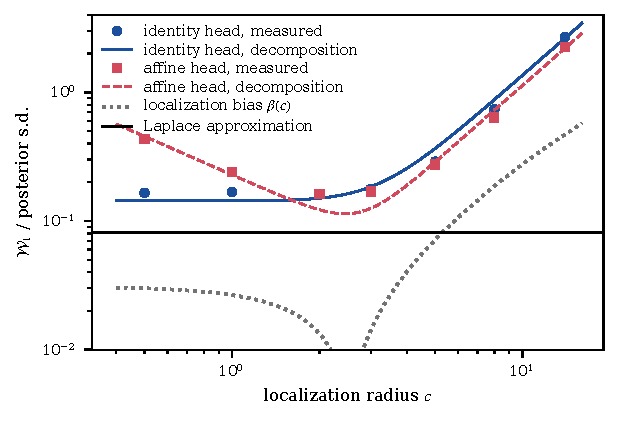
\includegraphics[width=0.9\textwidth]{mf_radius_theory}
\caption{The decomposition \eqref{m:eq:decomp} against measurement on the two dimensional Navier Stokes problem of Polson and Sokolov~\cite{polsonsokolov2026}, $D=6$, $M=1200$. Points are measured Wasserstein distances to an MCMC gold standard, in posterior standard deviations; curves are \eqref{m:eq:decomp} with $a_v$ and $b$ fitted separately for each head, and the bias $\beta(c)$ (dotted) is computed from \eqref{m:eq:bias} with no free parameter; the horizontal line is the Laplace approximation on the same run. The fitted optimum for the affine head is $c^\star=2.44$ against a measured optimum between $2$ and $3$; the root mean square residual of that fit is $0.044$. The localization bias is negligible below $c\approx3$, so in the fit of the affine head the left arm is estimation variance and the right arm nonlinearity. The identity head is the one produced by the study's script, whose residuals are neither centered at their sample mean nor rescaled, so that its flat left arm contains the displacement of Theorem~\ref{m:thm:locbias}(ii), which does not depend on $c$.}\label{m:fig:radius}
\end{figure}

Figure~\ref{m:fig:radius} tests \eqref{m:eq:decomp} on the Navier Stokes problem, with $a_v$ and $b$ fitted by least squares on the measured errors, which range from $0.16$ to $2.7$; the affine head's predicted optimum matches the measured one. The identity head's flat left arm is correctly predicted by $v=0$ (its level is mostly the displacement of Theorem~\ref{m:thm:locbias}(ii) and not the variance term), and the affine head's steep left arm by $v=2$: with a narrow proposal there is no design spread from which to estimate a slope.

\subsection{The design rule, and what it changes}

\begin{algorithm}[Localized GBC]\label{m:alg:loc}
Replace the step of Algorithm~\ref{m:alg:gbc} that simulates the training pairs by the following.
\begin{enumerate}[nosep]
\item Compute a preliminary estimate $\bar\theta_N$ and its Gauss Newton covariance $\Sigma_N$.
\item Draw $\theta^{(m)}\sim N(\bar\theta_N,c^2\Sigma_N)$ with $c\in[2,3]$, and simulate $Z^{(m)}$ from those.
\item Use the identity head with residuals centered at their sample mean (in the linear Gaussian model, equivalently, subtract $P\bar\theta_N$), and whiten by the sample covariance of the centered residuals rescaled by $(s_j+c^2p_j^2)^{-1/2}$ in the eigenbasis of $P$.
\item Do not add the residual mean to the center; do not use an affine head; do not importance weight back to the prior.
\end{enumerate}
\end{algorithm}

The radius $c\in[2,3]$ is not read off \eqref{m:eq:cstar}; the range is calibrated on the measurement, as Remark~\ref{m:rem:radiushead} sets out. Centering the residuals is Theorem~\ref{m:thm:locbias}(ii) and is the most consequential line of the algorithm; without it the generator carries a first order bias that no number of simulations removes. The rescaling is the second: without it the head reports the spread of the \emph{proposal} rather than of the posterior (Theorem~\ref{m:thm:locbias}(iii) and Remark~\ref{m:rem:rescale}). The prohibition on importance weighting is empirical and is explained by Theorem~\ref{m:thm:locbias}: the correction is unnecessary, because by Corollary~\ref{m:cor:locG}(i) there is no bias to remove once the residuals are centered and rescaled, while the weights $\pi/q_c$ are ratios of Gaussians with the wider density in the numerator and therefore have infinite variance whenever $c^2p_j\le1/2$ in some direction $j$, as in the data dominated directions here; in the Navier Stokes study the effective sample size never exceeded $34$ of $1200$ at any radius.

Algorithm~\ref{m:alg:loc} is a way of meeting (G1). Corollary~\ref{m:cor:locG} proves this in the linear Gaussian model. Localization is not new to the theory. The Bernstein von Mises theorems behind Theorem~\ref{m:thm:jwbvm} are proved on a localization set of the posterior, and Nickl and Wang~\cite{nicklwang2024}, in a steady state Schr\"odinger model, build their sampler on a surrogate log likelihood that agrees with the likelihood on a ball about a data driven initializer, of radius a small multiple of $D^{-4/d}$ with $D$ the dimension of their discretization, set by their stability estimate; only the training step had been left outside such a set.

\begin{corollary}[The localized design meets (G1) and (G2)]\label{m:cor:locG}
Consider the generator of Algorithm~\ref{m:alg:loc} with proposal $q_c=N(\bar\theta_N,c^2\Sigma_N)$ and $P=\Sigma_N\Sigma_0^{-1}$. In the setting of Lemma~\ref{m:lem:exact}, with $\Sigma_0$ and $\Phi^\top\Phi$ commuting as in Theorem~\ref{m:thm:locbias}:
\begin{enumerate}[label=(\roman*),nosep]
\item \emph{(Exactness in population.)} For every $c>0$ and every center $\bar\theta_N$, the law the head produces at the observed data is exactly the posterior, $N\big(S(Y),\Sigma_N\big)$. Localization contributes no bias at all, not merely a bias of smaller order.
\item \emph{(Finite $M$.)} With $M=M_N$ simulations and $J=J_N$ retained modes, the rescaled sample covariance of the centered residuals equals $\Sigma_N^{1/2}(\Id+\Delta_M)\Sigma_N^{1/2}$, where $\norm{\Delta_M}_{op}=O_P\big(\sqrt{J_N/M_N}+J_N/M_N\big)$ does not depend on $c$. Hence, when $\Sigma_{N,j}\lesssim\lambda_j/N$ on the retained modes ($\lambda_j$ the Laplace eigenvalues), as for the heat and Stokes equations, and $k>d/2$, $\Wone_{1,H^{-k-2}}(\Pihat,\PiN)=O_P\big(N^{-1/2}(\sqrt{J_N/M_N}+J_N/M_N)\big)$, so (G1) holds whenever $J_N/M_N\to0$, at every radius; and (G2) holds at every order whenever the exact posterior $N(S(Y),\Sigma_N)$ satisfies its first clause.
\item Consequently Theorem~\ref{m:thm:main} applies verbatim to Algorithm~\ref{m:alg:loc}, and Assumption~\ref{m:ass:G} is discharged for it.
\end{enumerate}
Part (i) does not use Assumption~\ref{m:ass:U}: in the linear Gaussian model the posterior given the summary is the posterior, so the two terms of Theorem~\ref{m:thm:qnnA} that need it vanish identically. Parts (ii) and (iii) quote the argument of Theorem~\ref{m:thm:qnnA}, and Remark~\ref{m:rem:u2pres} says what they need for a nonlinear forward map and what of it is open. Assumption~\ref{m:ass:u2p} itself is proved by Theorem~\ref{m:thm:u2ploc}, under the hypotheses there, for the uncentered and unrescaled head of Definition~\ref{m:def:gen}, so that Theorem~\ref{m:thm:qnnA} applies to that head under its other hypotheses.
\end{corollary}

\begin{proof}
(i) Write $A=\Sigma_NF$, so that $A+P=\Sigma_N(F+\Sigma_0^{-1})=\Id$, and $S=\Sigma_N\Phi^\top Y/\varsigma^2=A\theta+\Sigma_N\Phi^\top\varepsilon/\varsigma^2$. Hence
\[
R=\theta-S=P\theta-\Sigma_N\Phi^\top\varepsilon/\varsigma^2 ,
\]
which is Theorem~\ref{m:thm:locbias}: $E_{q_c}R=P\bar\theta_N$ and $\Var_{q_c}R=c^2P\Sigma_NP^\top+\Sigma_NF\Sigma_N$, equal to $\Sigma_{N,j}(s_j+c^2p_j^2)$ in the basis diagonalizing $P$. Subtracting the mean removes $P\bar\theta_N$ exactly, and dividing coordinate $j$ by $(s_j+c^2p_j^2)^{1/2}$ leaves variance exactly $\Sigma_{N,j}$; the rescaled residual is therefore $N(0,\Sigma_N)$, and the head returns $S(Y)+N(0,\Sigma_N)$, which by Lemma~\ref{m:lem:exact} is the exact posterior. What makes this work is not independence of $R$ and $S$, which fails under $q_c$: $\mathrm{Cov}_{q_c}(R,S)=(c^2P-\Id)\Sigma_NF\Sigma_N$, zero only when $c^2\Sigma_N=\Sigma_0$, as for the true prior. The head does not condition on $S$; it draws from the marginal law of the corrected residual and adds it to $S$, and that composition has the right conditional law because the corrected residual is $N(0,\Sigma_N)$ whatever $Y$ is.

(ii) Work in the basis diagonalizing $P$, $\Sigma_N$ and $F$, and let $V=\Var_{q_c}R$, diagonal with entries $\Sigma_{N,j}(s_j+c^2p_j^2)$ by (i). In the linear Gaussian model the residuals are $R^{(m)}=P\bar\theta_N+V^{1/2}g_m$ with $g_m$ i.i.d.\ $N(0,\Id_J)$, so the sample covariance of the centered residuals is $V^{1/2}(\Id+\Delta_M)V^{1/2}$, with $\Id+\Delta_M$ the sample covariance of the $g_m$; by the covariance estimation bound for Gaussian vectors~\cite[Theorem 4.7.1 and Exercise 4.7.3]{vershynin2018} with $u=J$, $\norm{\Delta_M}_{op}=O_P(\sqrt{J/M}+J/M)$, centering at the sample mean adding a term of rank one and of size $O_P(J/M)$. The rescaling is the diagonal matrix $Q$ with entries $(s_j+c^2p_j^2)^{-1/2}$, and $QV^{1/2}=\Sigma_N^{1/2}$, so the rescaled sample covariance is $\Sigma_N^{1/2}(\Id+\Delta_M)\Sigma_N^{1/2}$ and the radius drops out. The center of $\Pihat$ is $S(Y)$, as in (i), so coupling $\Pihat$ and $\PiN=N(S(Y),\Sigma_N)$ through a common $g\sim N(0,\Id_J)$ (Lemma~\ref{m:lem:coupling}) and using $|(1+x)^{1/2}-1|\le|x|$ for $x\ge-1$ gives
\[
\Wone_{1,H^{-k-2}}(\Pihat,\PiN)\le\big\|\Lambda^{-(k+2)/2}\Sigma_N^{1/2}\big\|_{HS}\,\norm{\Delta_M}_{op},
\]
where $\norm{\Lambda^{-(k+2)/2}\Sigma_N^{1/2}}^2_{HS}\le\sum_j\lambda_j^{-k-2}\Sigma_{N,j}\lesssim N^{-1}\sum_j\lambda_j^{-k-1}$ because $\Sigma_{N,j}\lesssim1/(N\iota_j)\lesssim\lambda_j/N$, and the sum is finite because $k>d/2$. For (G2), $\Pihat$ and $\PiN$ have the same center and the covariance of $\Pihat$ is at most $1+\norm{\Delta_M}_{op}$ times $\Sigma_N$, so the Gaussian concentration bounds in the proof of Theorem~\ref{m:thm:qnnA}, applied to either covariance, give spreads $O_P(r_N(s))$ in $H^s$. If $\PiN$ satisfies the first clause of (G2) with a constant $L$, then with probability above one half a draw from $\PiN$ lies in $\bar\Theta_{N,L}$, within $L\tilde\delta_N(0)$ of $S(Y)$ in $L^2$ and within $L$ of it in $H^{\bar\gamma}$, so $\norm{S(Y)-\theta_0}_{L^2}\le2L\tilde\delta_N(0)$ and $\norm{S(Y)}_{H^{\bar\gamma}}\le2L$ with probability tending to one, and the tail bound of that proof, with $L_1$ enlarged accordingly, gives (G2) for $\Pihat$ at every order.

(iii) is (i), (ii) and Theorem~\ref{m:thm:main}.
\end{proof}

\begin{remark}[Why the rescaling is not optional]\label{m:rem:rescale}
Without it the head reports $\sqrt{s_j+c^2p_j^2}$ times the correct posterior standard deviation in direction $j$, which is Theorem~\ref{m:thm:locbias}(iii). In the setting of Section~\ref{m:sec:expstudy}, $N=5\times10^4$ with $D=8$ retained modes of which $k_{\rm eff}=3$ are data dominated, the largest prior fraction is $p_{\max}=0.999$. The factor $\sqrt{1-p_j+c^2p_j^2}$ is at most one for every $p_j$ when $c=1$, so at that radius the unrescaled head \emph{understates} the posterior standard deviation, by at most $11\%$ over the eight modes, attained at $p_j=0.29$; for $c>1$ it overstates in every direction with $p_j>1/c^2$, by a factor that reaches $2.0$ at $c=2$, $3.0$ at $c=3$ and $8.0$ at $c=8$ in the most prior dominated direction.
\end{remark}

\begin{remark}[Which covariance the algorithm uses, and whether exactness survives it]\label{m:rem:whichcov}
$\Sigma_N$ in Algorithm~\ref{m:alg:loc} is $(F_{\bar\theta_N}+\Sigma_0^{-1})^{-1}$ with $F_{\bar\theta_N}$ the realized information $F_N$ of Remark~\ref{m:rem:reg}, that is the Gauss Newton information of the $N$ observations at the preliminary estimate, formed on the observed design. It is formed once and serves the proposal $c^2\Sigma_N$, the eigenbasis of $P$, and the factors $(s_j+c^2p_j^2)^{-1/2}$ alike; it is not reevaluated at the training draws, which is what keeps the cost at one Gauss Newton solve rather than $M$.

In the linear model nothing is plugged in, since $F=\Phi^\top\Phi/\varsigma^2$ does not depend on the point of evaluation; Corollary~\ref{m:cor:locG}(i) holds as stated. Nonlinearly it is a plug in and (i) does not survive verbatim. One thing does: one matrix serves both the proposal and the rescaling, so for the linearized residuals the correction $(s_j+c^2p_j^2)^{-1/2}$ undoes the inflation that produced them whatever $F_{\bar\theta_N}$ is. Two errors are left over. One is the discrepancy between $\Sigma_N(\bar\theta_N)$ and the Bernstein von Mises covariance, the same plug in error of order $\tilde\delta_N(\zeta)$ that Section~\ref{m:sec:qnn} bounds under the Lipschitz clause (U3). The other is the nonlinear remainder of the residuals under $q_c$, which Proposition~\ref{m:prop:locres} controls for a reused design. Granted the hypotheses that Remark~\ref{m:rem:u2pres} lists for parts (ii) and (iii), both enter (G1) additively alongside the $\sqrt{J_N/M_N}$ of (ii), and what is lost is the sharper reading of (i), that localization costs nothing at all rather than something of smaller order.
\end{remark}

\begin{remark}[The remaining term]\label{m:rem:relin}
In \eqref{m:eq:decomp} the term $b\,c^4$ arises because the summary is linearized once, at $\bar\theta_N$. Lemma~\ref{m:lem:exact} says that in the linear model the summary does not depend on the linearization point at all; the $c^4$ term is therefore purely a nonlinear effect, and it can be removed by iterating the Gauss Newton step and recomputing the Jacobian from the data alone at each iterate instead of once at $\bar\theta_N$, at a cost of $D+1$ forward solves per training draw for each extra step. Recomputing it at the training parameter $\theta^{(m)}$ would not define a statistic, since that parameter is not available for the observed data. The decomposition then reduces to $\beta(c)^2+a_v/c^v$, which for the affine head decreases in $c$ until the bias $\beta(c)$ begins to grow, so the optimal radius moves out to where the localization bias binds, and the achievable error is within $O(\sqrt{D/M})$ of the smallest value of $\beta(c)$, the floor it approaches as $M$ grows. Polson and Sokolov~\cite{polsonsokolov2026} carried this out with a two step Gauss Newton summary and confirmed that the $c^4$ term disappears; the error of the affine head at $c=6$ fell from $0.37$ to $0.16$ and became flat in $c$. After centering, the localized GBC posterior and the Laplace approximation agree with each other and with a $4500$ sample MCMC reference to the reference's own Monte Carlo error, $0.06$ posterior standard deviations. The cubic correction to the center, the first order shift $\frac12H^{-1}g$ of the posterior mean from the maximum a posteriori estimate, where $H$ is the negative Hessian of the log posterior density $\ell$ at the maximum and $g_a=\sum_{b,c}(H^{-1})_{bc}\,\partial_a\partial_b\partial_c\ell$ there, is at most $0.01$ standard deviations there, so the posterior is Gaussian in its center to that accuracy and neither method has anything left to correct in the well specified $T_0=0$ regime.
\end{remark}

\subsection{The whitened residuals of a localized proposal}\label{m:sec:u2ploc}

Everything is conditional on the data: $P$, $E$ and $\norm\cdot_{\psi_2}$ refer to the draw of the training pairs with $Z^{(N)}$ fixed, unless $P^\N_{\theta_0}$ is written. A simulated data set $Z^{(m)}$ is drawn from \eqref{m:eq:model} at $\theta^{(m)}$, with its own design points $X^{(m)}_i$, uniform on $\mathcal X$, and its own noise $\varepsilon^{(m)}_i\sim N(0,I_W)$, independent of each other and of $\theta^{(m)}$.

\emph{Notation.} Write $X$ for a uniform point of $\mathcal X$, $d_W$ for the dimension of an observation, $E_J=\mathrm{span}\{e_j:j\le J\}$, identified with $\R^J$, $P_J$ for the orthogonal projection onto it, $Q_J=\Id-P_J$, and $J=J_N$, so that $p_N=P_J$ in \eqref{m:eq:summary}. For a linear map $\mathcal T$ from $\ell^2$ into $\R^{d_W}$ valued functions on $\mathcal X$ let $\norm{\mathcal T}_{\ell^2\to L^2}=\sup_{\norm g_2\le1}(E\norm{(\mathcal Tg)(X)}^2_W)^{1/2}$. At a point $\vartheta$ where the linearization $\I_\vartheta$ is defined, define $K'_\vartheta$ by
\begin{equation}\label{m:eq:u2pF}
\langle f,(\Id+K'_\vartheta)g\rangle=E\big\langle(\I_\vartheta\mathcal D^{1/2}f)(X),(\I_\vartheta\mathcal D^{1/2}g)(X)\big\rangle_W ,
\end{equation}
that is $\Id+K'_\vartheta=T^{-1}\mathcal D^{1/2}\I^*_\vartheta\I_\vartheta\mathcal D^{1/2}$. Then $K'_{\theta_0}=K'$, $\norm{\I_\vartheta\mathcal D^{1/2}}^2_{\ell^2\to L^2}=\norm{\Id+K'_\vartheta}_{op}$, and $\Id+\Xi_\vartheta=P_J(\Id+K'_\vartheta)^{-1}P_J$. Fix a linearization point $\bar\vartheta$ determined by $Z^{(N)}$ at which $\Id+K'_{\bar\vartheta}$ is bounded and invertible, and let the training summary be \eqref{m:eq:summary} with one fold and the linearization point held at $\bar\vartheta$. It is linearized once, as in Remark~\ref{m:rem:relin}, but it uses the population information and carries no prior term, unlike the regularized summary of Lemma~\ref{m:lem:exact}: for $j\le J$,
\begin{equation}\label{m:eq:trainsummary}
\begin{aligned}
\hat S^{(m)}_{N,j}&=\langle e_j,\bar\vartheta\rangle\\
&\quad+\frac1N\sum_{i\le N}\Big\langle\I_{\bar\vartheta}\,p_N\big(\bar e_j^{\,\bar\vartheta}\big)(X^{(m)}_i),\;Y^{(m)}_i-u_{\bar\vartheta}(X^{(m)}_i)\Big\rangle_W .
\end{aligned}
\end{equation}
Since $\bar e_j^{\,\vartheta}=\mathcal D^{1/2}(\Id+K'_\vartheta)^{-1}\mathcal D^{1/2}e_j$ and $\mathcal D$ commutes with $P_J$, the whitened weights $\phi_j(x)=\iota_j^{1/2}\,\I_{\bar\vartheta}p_N(\bar e_j^{\,\bar\vartheta})(x)\in\R^{d_W}$ satisfy
\begin{equation}\label{m:eq:u2pW}
\sum_{j\le J}v_j\phi_j(x)=\big(\I_{\bar\vartheta}\mathcal D^{1/2}P_J(\Id+K'_{\bar\vartheta})^{-1}v\big)(x),\qquad v\in\R^J .
\end{equation}
Let $\phi(x)$ be the $J\times d_W$ matrix with rows $\phi_j(x)^\top$, so that the left side of \eqref{m:eq:u2pW} is $\phi(x)^\top v$, and write
\[
\begin{gathered}
G_\phi=E\,\phi(X)\phi(X)^\top,\qquad\hat G^{(m)}_\phi=\frac1N\sum_{i\le N}\phi(X^{(m)}_i)\phi(X^{(m)}_i)^\top,\\
b_J=\mathrm{ess\,sup}_x\norm{\phi(x)}^2_{op}
\end{gathered}
\]
for the Gram matrix of the whitened weights, its realized version and its envelope. Since $\norm{\phi\phi^\top}_F\le\norm\phi_{op}\norm\phi_F$, Chebyshev's inequality gives, for $t>0$ and the realized Gram matrix $\hat G_\phi$ of any $N$ independent uniform points of $\mathcal X$,
\begin{equation}\label{m:eq:u2pcheb}
\begin{aligned}
P\big(\norm{\hat G_\phi-G_\phi}_{op}>t\big)&\le t^{-2}E\norm{\hat G_\phi-G_\phi}^2_F\\
&\le\frac{E\norm{\phi(X)\phi(X)^\top}^2_F}{Nt^2}\le\frac{b_J\tr G_\phi}{Nt^2} .
\end{aligned}
\end{equation}
Substituting $Y^{(m)}_i=u_{\theta^{(m)}}(X^{(m)}_i)+\varepsilon^{(m)}_i$ in \eqref{m:eq:trainsummary} gives, for $v\in\R^J$,
\begin{equation}\label{m:eq:u2pdecomp}
\langle v,W^{(m)}\rangle=\mu_v-\frac1{\sqrt N}\sum_{i\le N}\big\langle\phi(X^{(m)}_i)^\top v,\varepsilon^{(m)}_i\big\rangle_W ,
\end{equation}
with $\mu_v$ a function of $Z^{(N)}$, $\theta^{(m)}$ and the design, so that conditionally on these $\langle v,W^{(m)}\rangle$ is normal with variance $v^\top\hat G^{(m)}_\phi v$.

\begin{lemma}[The Gram matrix of the whitened weights]\label{m:lem:u2pgram}
Let $\mathcal A=\Id+K'_{\bar\vartheta}$ be bounded on $\ell^2$ with $\mathcal A\succeq a\Id$ for some $a>0$, and write $B_J=\Id+\Xi_{\bar\vartheta}=P_J\mathcal A^{-1}P_J$. Then
\[
G_\phi=B_J+B_JP_J\mathcal AQ_J(Q_J\mathcal AQ_J)^{-1}Q_J\mathcal AP_JB_J ,
\]
so that $G_\phi\succeq B_J\succeq\norm{\mathcal A}^{-1}_{op}\Id$ and $\norm{G_\phi-B_J}_{op}\le a^{-3}\norm{K'_{\bar\vartheta}Q_J}^2_{op}$.
\end{lemma}

\begin{proof}
By \eqref{m:eq:u2pW} and \eqref{m:eq:u2pF}, $G_\phi=B_JP_J\mathcal AP_JB_J$ on $E_J$, and block inversion of $\mathcal A$ on $E_J\oplus Q_J\ell^2$ gives $B_J^{-1}=P_J\mathcal AP_J-P_J\mathcal AQ_J(Q_J\mathcal AQ_J)^{-1}Q_J\mathcal AP_J$; substituting gives the display, whose second term is positive semidefinite. Also $\mathcal A^{-1}\succeq\norm{\mathcal A}^{-1}_{op}\Id$, $\norm{Q_J\mathcal AP_J}_{op}=\norm{Q_JK'_{\bar\vartheta}P_J}_{op}\le\norm{K'_{\bar\vartheta}Q_J}_{op}$ by self adjointness, and $\norm{B_J}_{op}$ and $\norm{(Q_J\mathcal AQ_J)^{-1}}_{op}$ are at most $a^{-1}$.
\end{proof}

\begin{proposition}[No sub Gaussian envelope for the whole residual]\label{m:prop:u2pfalse}
Let each simulated data set have its own design, as in \eqref{m:eq:model}, let the training summary be \eqref{m:eq:trainsummary}, and let the training parameters have any law given $Z^{(N)}$. Then for every $N$, every $J$ and every unit vector $v\in\R^J$
\[
\begin{gathered}
\big\|\langle v,W^{(m)}\rangle\big\|^2_{\psi_2\mid Z^{(N)}}\ge2\,\mathrm{ess\,sup}_x\norm{\phi(x)^\top v}^2_W ,\\
\sup_{\norm u_2=1}\big\|\langle u,W^{(m)}\rangle\big\|^2_{\psi_2\mid Z^{(N)}}\ge2b_J\ge\frac{2\tr G_\phi}{d_W} .
\end{gathered}
\]
If $\Id+K'_{\bar\vartheta}$ is bounded and $\Id+K'_{\bar\vartheta}\succeq a\Id$ for some $a>0$, then $\tr G_\phi\ge J\norm{\Id+K'_{\bar\vartheta}}^{-1}_{op}$. For the heat and Stokes equations, observed from time zero as in \eqref{m:eq:model}, $G_\phi=\Id_J$ and $\norm{\langle e_J,W^{(m)}\rangle}^2_{\psi_2\mid Z^{(N)}}\ge2\norm{e_J}^2_{L^\infty}/\iota_J\ge2/\iota_J$, which grows like $\lambda_J$ by \eqref{m:eq:iota}; for the real trigonometric basis the bound is $4/\iota_J$.
\end{proposition}

\begin{proof}
Fix a unit vector $v$ and $s^2<\mathrm{ess\,sup}_x\norm{\phi(x)^\top v}^2_W$. The set $\mathcal X_s=\{x:\norm{\phi(x)^\top v}^2_W>s^2\}$ has positive measure, so with probability $P(X\in\mathcal X_s)^N>0$, whatever $\theta^{(m)}$ is, all $N$ design points lie in it, and then the conditional variance $\sigma^2=v^\top\hat G^{(m)}_\phi v$ in \eqref{m:eq:u2pdecomp} exceeds $s^2$. For $K^2<2s^2$ the exponent of $e^{x^2/K^2-(x-\mu_v)^2/(2\sigma^2)}$ then has a positive coefficient of $x^2$, so the conditional expectation of $e^{\langle v,W^{(m)}\rangle^2/K^2}$ given $Z^{(N)}$, $\theta^{(m)}$ and the design is infinite on an event of positive probability, and $\norm{\langle v,W^{(m)}\rangle}^2_{\psi_2\mid Z^{(N)}}\ge2s^2$. This is the first inequality. For the second, let $(v_k)$ be dense in the unit sphere of $\R^J$ and $c<b_J$. Each $x$ in the set $\{x:\norm{\phi(x)}^2_{op}>c\}$, which has positive measure, has $\norm{\phi(x)^\top v_k}^2_W>c$ for some $k$, so for some $k$ the set of such $x$ has positive measure, and the first inequality with $v=v_k$ gives $2c$. Next, $\norm{\phi(x)}^2_{op}\ge\norm{\phi(x)}^2_F/d_W$ and $\mathrm{ess\,sup}_x\norm{\phi(x)}^2_F\ge E\norm{\phi(X)}^2_F=\tr G_\phi$, and $\tr G_\phi\ge\tr(\Id+\Xi_{\bar\vartheta})\ge J\norm{\Id+K'_{\bar\vartheta}}^{-1}_{op}$ by Lemma~\ref{m:lem:u2pgram}. For the heat and Stokes equations $\I_\vartheta=\Lcal$ and $\Kcal=0$ in \eqref{m:eq:fredholm}, so $K'_{\bar\vartheta}=0$, $G_\phi=\Id_J$, and $\phi(t,x)^\top e_J=\iota_J^{-1/2}e^{-\nu\lambda_Jt}e_J(x)$ by \eqref{m:eq:modeinfo}, a continuous function whose squared norm has supremum $\norm{e_J}^2_{L^\infty}/\iota_J$, at $t=0$. The first inequality with $v=e_J$ gives the bound, and $\norm{e_J}^2_{L^\infty}\ge\int_\Omega\norm{e_J}^2_W=1$.
\end{proof}

For a nonlinear forward map three conditions on the linearization take the place of the explicit structure of the heat equation, and a fourth bounds its remainder. They involve a constant $a_\star>0$ and, for every $B>0$, constants $L_\star$, $C_\infty$ and $C_Q$ that may depend on $B$, and they are required for all $\vartheta,\vartheta'$ with $\norm\vartheta_{H^{\bar\gamma}},\norm{\vartheta'}_{H^{\bar\gamma}}\le B$:
\begin{enumerate}[label=(I\arabic*),nosep]
\item $\Id+K'_{\theta_0}$ is bounded on $\ell^2$, $K'_{\theta_0}$ is compact, and $\Id+K'_{\theta_0}\succeq a_\star\Id$;
\item $\norm{(\I_\vartheta-\I_{\theta_0})\mathcal D^{1/2}}_{\ell^2\to L^2}\le L_\star\norm{\vartheta-\theta_0}_{H^\zeta}$;
\item $\norm{\I_\vartheta h}_{L^\infty(\mathcal X)}\le C_\infty\norm h_{H^\zeta}$ for all $h\in H^\zeta$;
\item $\norm{u_{\vartheta'}-u_\vartheta-\I_\vartheta[\vartheta'-\vartheta]}_{L^\infty(\mathcal X)}\le C_Q\norm{\vartheta'-\vartheta}^2_{H^\zeta}$.
\end{enumerate}
Condition (I2) is a Lipschitz bound in the whitened $H^{-1}$ metric. It gives $\norm{\Xi_\vartheta-\Xi_{\theta_0}}_{op}\lesssim\norm{\vartheta-\theta_0}_{H^\zeta}$ for $\vartheta$ near $\theta_0$, uniformly in $J$, which the weight condition \eqref{m:eq:lipweight} does not, since its factor $\norm{e_j}_{H^{\kappa+2}}$ grows with $j$. Condition (I3) at $\vartheta=\theta_0$ is the second part of Condition 2D of Nickl~\cite{nicklbvm2024}. For Navier Stokes, (I1) is shown before Assumption~\ref{m:ass:u2p}, and Lemma~\ref{m:lem:nslin} proves (I2) to (I4).

\begin{theorem}[Assumption~\ref{m:ass:u2p} under a localized proposal]\label{m:thm:u2ploc}
Let $\bar\theta_N$ be a preliminary estimate as in Definition~\ref{m:def:summary}, let $J=J_N\asymp N^{d/(2\gamma+d)}$, and let the training parameters be
\[
\theta^{(m)}=\bar\theta_N+N^{-1/2}\mathcal D^{1/2}\mathcal V_N^{1/2}\xi^{(m)},
\]
where $\mathcal V_N$ is a positive semidefinite $J\times J$ matrix determined by $Z^{(N)}$ with $\norm{\mathcal V_N}_{op}=O_P(1)$, and the $\xi^{(m)}$ are i.i.d.\ standard normal on $\R^J$ given $Z^{(N)}$, conditioned on $\norm{\xi^{(m)}}^2_2\le4J$ when the forward map is nonlinear. Let the training summary be \eqref{m:eq:trainsummary} with $\bar\vartheta=\bar\theta_N$, and the generator that of Definition~\ref{m:def:gen}, uncentered and unrescaled.
\begin{enumerate}[label=(\alph*),nosep]
\item For the heat and Stokes equations, observed from time zero as in \eqref{m:eq:model}, with $\gamma>d+2$, which the hypotheses of Theorem~\ref{m:thm:qnnA} imply, Assumption~\ref{m:ass:u2p} holds with $\Xi=0$, $\varkappa_N\le4/\sqrt3$ and $W^{(m)}_{\rm g}=-1_{\mathcal B_m}N^{-1/2}\sum_i\phi(X^{(m)}_i)\varepsilon^{(m)}_i$, where $\mathcal B_m=\{\norm{\hat G^{(m)}_\phi-\Id}_{op}\le1\}$.
\item For a nonlinear forward map, Assumption~\ref{m:ass:u2p} holds under Conditions 1 and 2 of Nickl~\cite{nicklbvm2024} with the constants of Theorem~\ref{m:thm:nickl2}, $\bar\gamma<\gamma-1$, the rate hypothesis $\sqrt N\,\tilde\delta_N(0)\tilde\delta_N(\zeta)\to0$ of Proposition~\ref{m:prop:suff}, and (I1) to (I3).
\item Let $\Sigma_0$ be positive definite, $\Sigma_N=(F_{\bar\theta_N}+\Sigma_0^{-1})^{-1}$ with $F_{\bar\theta_N}$ the realized information on $J$ modes (Remark~\ref{m:rem:whichcov}), and $a_\star=1$ in (a). Under the hypotheses of (a) or (b), with probability tending to one $N^{-1}\mathcal D^{1/2}F_{\bar\theta_N}\mathcal D^{1/2}\succeq(a_\star/12)\Id$, and then $\mathcal V_N=c^2N\mathcal D^{-1/2}\Sigma_N\mathcal D^{-1/2}$ has $\norm{\mathcal V_N}_{op}\le12c^2/a_\star$.
\end{enumerate}
\end{theorem}

The proposal $N(\bar\theta_N,c^2\Sigma_N)$ of Algorithm~\ref{m:alg:loc} on $D=J$ modes has this form with $\mathcal V_N=c^2N\mathcal D^{-1/2}\Sigma_N\mathcal D^{-1/2}$, and part (c) gives $\norm{\mathcal V_N}_{op}=O_P(1)$. For the heat and Stokes equations $N^{-1}\mathcal D^{1/2}F_{\bar\theta_N}\mathcal D^{1/2}$ is the realized Gram matrix $\hat G_\phi$ of the observed design, which tends to $\Id$ by \eqref{m:eq:u2pcheb}, since $b_JJ/N\to0$ (Step 5 below). Since $P(\norm\xi^2_2>4J)\le(4e^{-3})^{J/2}$, truncated and untruncated draws coincide except on an event of probability at most $M(4e^{-3})^{J/2}$, which tends to zero when $\log M_N=o(J_N)$. If instead the simulated data sets reuse the observed design $(X_i)_{i\le N}$ and draw only fresh noise, as in Lemma~\ref{m:lem:exact}, then for the heat and Stokes equations the computation of Step 1 below gives $W^{(m)}=-(\hat G_\phi-\Id)\mathcal V_N^{1/2}\xi^{(m)}-N^{-1/2}\sum_i\phi(X_i)\varepsilon^{(m)}_i$, which is centered Gaussian given $Z^{(N)}$ with covariance $(\hat G_\phi-\Id)\mathcal V_N(\hat G_\phi-\Id)+\hat G_\phi$. Since $\hat G_\phi\to\Id$, Assumption~\ref{m:ass:u2p} then holds with $W^{(m)}_{\rm r}=0$, and the whole residual has a sub Gaussian norm bounded uniformly in $J$ with probability tending to one.

\begin{proof}
In (a) the bounds below depend on $Z^{(N)}$ only through $\norm{\mathcal V_N}_{op}$. In (b) the events $A_N$ on which $\norm{\mathcal V_N}_{op}\le c_{\mathcal V}$, $\norm{\bar\theta_N}_{H^{\bar\gamma}}\le B$, $\norm{\bar\theta_N-\theta_0}_{H^\zeta}\le L\tilde\delta_N(\zeta)$ and $\norm{\bar\theta_N-\theta_0}_{L^2}\le L\tilde\delta_N(0)$ have probability tending to one as $c_{\mathcal V},B,L\to\infty$, uniformly in large $N$, by Definition~\ref{m:def:summary}. Let $\eta_N$ be the sum of the two quantities in the second display of Assumption~\ref{m:ass:u2p}. It suffices to show that for fixed constants, with $Z^{(N)}$ fixed, $\norm{\mathcal V_N}_{op}\le c_{\mathcal V}$ in (a) and $A_N$ in force in (b), $\varkappa_N$ is bounded and $\eta_N$ is at most a deterministic sequence that tends to zero. We drop the index $m$.

\emph{Step 1: decomposition.} Write $\mathcal A=\Id+K'_{\bar\theta_N}$, $\mathcal A_0=\Id+K'_{\theta_0}$, $\tilde h=\mathcal V_N^{1/2}\xi\in E_J$, $h=\theta-\bar\theta_N=N^{-1/2}\mathcal D^{1/2}\tilde h$ and $\tilde u=\I_{\theta_0}\mathcal D^{1/2}\tilde h$. With $R_0(\vartheta)=u_\vartheta-u_{\theta_0}-\I_{\theta_0}[\vartheta-\theta_0]$ we have $u_\theta-u_{\bar\theta_N}=N^{-1/2}\tilde u+r_\theta$, where $r_\theta=R_0(\theta)-R_0(\bar\theta_N)$ vanishes for a linear map, and substituting $Y_i=u_\theta(X_i)+\varepsilon_i$ in \eqref{m:eq:trainsummary} gives
\[
\begin{aligned}
W&=\tilde h-\frac1N\sum_i\phi(X_i)\tilde u(X_i)\\
&\quad-\frac1{\sqrt N}\sum_i\phi(X_i)r_\theta(X_i)-\frac1{\sqrt N}\sum_i\phi(X_i)\varepsilon_i .
\end{aligned}
\]
By \eqref{m:eq:u2pW}, the summands of the first sum have mean $P_J\mathcal A^{-1}P_JT^{-1}\mathcal D^{1/2}\I^*_{\bar\theta_N}\I_{\theta_0}\mathcal D^{1/2}\tilde h$ over $X$, and writing $\tilde h=P_J\mathcal A^{-1}\mathcal A\tilde h$ with $Q_J\mathcal A\tilde h=Q_JK'_{\bar\theta_N}\tilde h$ shows that $\tilde h$ minus this mean is $\mathcal C\tilde h$, where
\[
\mathcal C=P_J\mathcal A^{-1}Q_JK'_{\bar\theta_N}P_J+P_J\mathcal A^{-1}P_JT^{-1}\mathcal D^{1/2}\I^*_{\bar\theta_N}\big(\I_{\bar\theta_N}-\I_{\theta_0}\big)\mathcal D^{1/2}P_J .
\]
With the design event $\mathcal B=\{\norm{\hat G_\phi-G_\phi}_{op}\le1\}$ set
\[
\begin{aligned}
W_{\rm g}&=\mathcal C\tilde h-1_{\mathcal B}\frac1{\sqrt N}\sum_i\phi(X_i)\varepsilon_i ,\\
W_{\rm r}&=-1_{\mathcal B^c}\frac1{\sqrt N}\sum_i\phi(X_i)\varepsilon_i-\Big(\frac1N\sum_i\phi(X_i)\tilde u(X_i)-E\,\phi(X)\tilde u(X)\Big)\\
&\quad-\frac1{\sqrt N}\sum_i\phi(X_i)r_\theta(X_i),
\end{aligned}
\]
the expectation in the middle term taken over $X$ with $\tilde h$ fixed. Then $W=W_{\rm g}+W_{\rm r}$, the pairs $(W_{\rm g},W_{\rm r})$ are i.i.d.\ over the simulations given $Z^{(N)}$, and $E\,W_{\rm g}=0$, because $\xi$ is symmetric and the noise is centered and independent of $\xi$ and of the design.

\emph{Step 2: the sub Gaussian part.} Given the design and $\xi$, the variable $1_{\mathcal B}N^{-1/2}\sum_i\langle\phi(X_i)^\top v,\varepsilon_i\rangle_W$ is centered normal with variance at most $s^2=\norm{G_\phi}_{op}+1$ for unit $v$, and a centered normal variable $\chi$ with variance at most $s^2$ has $E\,e^{\chi^2/K^2}\le(1-2s^2/K^2)^{-1/2}=2$ at $K^2=8s^2/3$, so its sub Gaussian norm is at most $(8/3)^{1/2}s$. For the other term, $\langle v,\mathcal C\tilde h\rangle=\langle\mathcal V_N^{1/2}\mathcal C^\top v,\xi\rangle$, and every $\langle u,\xi\rangle$ with $\norm u_2=1$ has sub Gaussian norm at most $2\sqrt3$: $E\,e^{\langle u,\xi\rangle^2/12}=(5/6)^{-1/2}$ for the standard normal law, and conditioning on $\{\norm\xi^2_2\le4J\}$, an event of probability at least $1-(4e^{-3})^{J/2}\ge0.55$ by the Chernoff bound $P(\norm\xi^2_2\ge4J)\le e^{-3J/2}E\,e^{3\norm\xi^2_2/8}$, raises this to at most $(5/6)^{-1/2}/0.55<2$. Hence
\[
\varkappa_N\le(8/3)^{1/2}\big(\norm{G_\phi}_{op}+1\big)^{1/2}+2\sqrt3\,c_{\mathcal V}^{1/2}\norm{\mathcal C}_{op} .
\]

\emph{Step 3: the second moment.} The two terms of $W_{\rm g}$ are uncorrelated, since the second is centered given $\xi$ and the design, and $E\,\xi\xi^\top\preceq\Id$, since the truncation preserves rotation invariance and does not raise $E\norm\xi^2_2$. Hence $E\,W_{\rm g}W_{\rm g}^\top=E\,\mathcal C\tilde h\tilde h^\top\mathcal C^\top+G_\phi-E\,\hat G_\phi1_{\mathcal B^c}$, where the first term has norm at most $c_{\mathcal V}\norm{\mathcal C}^2_{op}$ and the last at most $b_JP(\mathcal B^c)\le b_J^2\tr G_\phi/N$ by \eqref{m:eq:u2pcheb}. With Lemma~\ref{m:lem:u2pgram}, $a$ a lower bound for $\mathcal A$, and $\norm{\Xi_{\bar\theta_N}-\Xi_{\theta_0}}_{op}\le\norm{\mathcal A^{-1}-\mathcal A_0^{-1}}_{op}$, this gives
\[
\begin{aligned}
\big\|E\,W_{\rm g}W_{\rm g}^\top-(\Id+\Xi)\big\|_{op}&\le c_{\mathcal V}\norm{\mathcal C}^2_{op}+\frac{b_J^2\tr G_\phi}N\\
&\quad+\frac{\norm{K'_{\bar\theta_N}Q_J}^2_{op}}{a^3}+\norm{\mathcal A^{-1}-\mathcal A_0^{-1}}_{op} .
\end{aligned}
\]

\emph{Step 4: the remainder.} Given the design, the first term of $W_{\rm r}$ has second moment $1_{\mathcal B^c}\tr\hat G_\phi\le1_{\mathcal B^c}d_Wb_J$. Given $\xi$, the middle term is an average of $N$ i.i.d.\ centered vectors, with second moment at most $N^{-1}E\norm{\phi(X)}^2_{op}\norm{\tilde u(X)}^2_W\le N^{-1}b_J\langle\tilde h,\mathcal A_0\tilde h\rangle$. Given $\theta$, the last term has second moment at most $E\norm{\phi(X)r_\theta(X)}^2_2+N\norm{E\,\phi(X)r_\theta(X)}^2_2\le(b_J+N\norm{G_\phi}_{op})E\norm{r_\theta(X)}^2_W$, because $\norm{E\,\phi r_\theta}_2=\sup_{\norm v_2=1}E\langle\phi^\top v,r_\theta\rangle_W\le\norm{G_\phi}^{1/2}_{op}(E\norm{r_\theta}^2_W)^{1/2}$. With \eqref{m:eq:u2pcheb} and $E\norm{\tilde h}^2_2\le c_{\mathcal V}J$ this gives
\[
\begin{aligned}
E\norm{W_{\rm r}}^2_2&\le\frac{3d_Wb_J^2\tr G_\phi}N+\frac{3c_{\mathcal V}b_J\norm{\mathcal A_0}_{op}J}N\\
&\quad+3\big(b_J+N\norm{G_\phi}_{op}\big)\sup_\theta E\norm{r_\theta(X)}^2_W ,
\end{aligned}
\]
the supremum taken over the support of the proposal.

\emph{Step 5: the heat and Stokes equations.} Here $K'_\vartheta=0$, $\I_\vartheta=\Lcal$ and $r_\theta=0$, so $\mathcal C=0$, $\mathcal A=\mathcal A_0=G_\phi=\Id$, $\Xi=0$ and $\varkappa_N\le(16/3)^{1/2}=4/\sqrt3$. The weights are $\phi_j(t,x)=\iota_j^{-1/2}e^{-\nu\lambda_jt}e_j(x)$ with $\norm{e_j(x)}^2_W\le2$, and $\iota_j^{-1}\le1+2\nu\lambda_jT$ by \eqref{m:eq:iota} at $T_0=0$, so $b_J\le2\sum_{j\le J}\iota_j^{-1}\lesssim J\lambda_J\asymp J^{1+2/d}$. Steps 3 and 4 bound $\eta_N$ by a constant times $b_J^2J/N\lesssim N^{(3d+4)/(2\gamma+d)-1}$, which tends to zero because $\gamma>d+2$. The hypotheses of Theorem~\ref{m:thm:qnnA} give $\gamma>3\zeta+3d/2+2$ with $\zeta>d/2$, hence $\gamma>3d+2$. This proves (a).

\emph{Step 6: a nonlinear map.} By (I2), $\upsilon_N=\norm{(\I_{\bar\theta_N}-\I_{\theta_0})\mathcal D^{1/2}}_{\ell^2\to L^2}\le L_\star L\tilde\delta_N(\zeta)\to0$. Since $\mathcal A-\mathcal A_0$ is the difference of the forms \eqref{m:eq:u2pF} at $\bar\theta_N$ and at $\theta_0$, $\norm{\mathcal A-\mathcal A_0}_{op}\le\upsilon_N(2\norm{\mathcal A_0}^{1/2}_{op}+\upsilon_N)\to0$, so for $N$ large $\mathcal A\succeq(a_\star/2)\Id$, $\norm{\mathcal A^{-1}-\mathcal A_0^{-1}}_{op}\le2a_\star^{-2}\norm{\mathcal A-\mathcal A_0}_{op}\to0$, and $\norm{K'_{\bar\theta_N}Q_J}_{op}\le\norm{K'_{\theta_0}Q_J}_{op}+\norm{\mathcal A-\mathcal A_0}_{op}\to0$, the first term because $K'_{\theta_0}$ is compact and self adjoint by (I1). Since $P_J\mathcal A^{-1}Q_J=-P_J\mathcal A^{-1}K'_{\bar\theta_N}Q_J$,
\[
\norm{\mathcal C}_{op}\le\frac2{a_\star}\Big(\norm{K'_{\bar\theta_N}Q_J}^2_{op}+\norm{\mathcal A}^{1/2}_{op}\,\upsilon_N\Big)\to0 ,
\]
while $\norm{G_\phi}_{op}\le2/a_\star+8a_\star^{-3}\norm{K'_{\bar\theta_N}Q_J}^2_{op}$ stays bounded by Lemma~\ref{m:lem:u2pgram}, so $\varkappa_N$ is bounded. By (I3) and \eqref{m:eq:u2pW}, $\norm{\phi(x)^\top v}_W\le C_\infty\norm{\mathcal D^{1/2}P_J\mathcal A^{-1}v}_{H^\zeta}\le C_\infty(2/a_\star)\max_{j\le J}(1+\lambda_j)^{\zeta/2}\iota_j^{-1/2}\norm v_2$, so $b_J\lesssim\lambda_J^{\zeta+1}$ and $b_J^2J/N\lesssim N^{(4\zeta+4+d)/(2\gamma+d)-1}\to0$, because $\gamma>3\zeta+3d/2+2>2\zeta+2$ by the hypotheses of Theorem~\ref{m:thm:nickl2}. It remains to bound $r_\theta$. On the support of the proposal, for $s\ge0$,
\[
\norm h^2_{H^s}\le\frac{4c_{\mathcal V}J}N\max_{j\le J}(1+\lambda_j)^s\iota_j^{-1}\lesssim\frac{J\lambda_J^{s+1}}N ,
\]
which tends to zero for $s=\bar\gamma$ because $\bar\gamma<\gamma-1$. So for $N$ large both $\theta-\theta_0$ and $\bar\theta_N-\theta_0$ lie in $U(\bar\gamma,B+\norm{\theta_0}_{H^{\bar\gamma}}+1)$, and Condition 2C, applied to each of the two terms of $r_\theta$, gives
\[
\big(E\norm{r_\theta(X)}^2_W\big)^{1/2}\lesssim\norm{\theta-\theta_0}^2_{L^2}+\norm{\bar\theta_N-\theta_0}^2_{L^2}\lesssim\tilde\delta_N(0)^2+\frac{J\lambda_J}N .
\]
Since $\tilde\delta_N(0)\le\tilde\delta_N(\zeta)$, the rate hypothesis gives $N\tilde\delta_N(0)^4\to0$, and $N(J\lambda_J/N)^2\asymp N^{(2d+4)/(2\gamma+d)-1}\to0$ because $\gamma>2+d/2$; also $b_J\lesssim N$. Steps 2 to 4 now give (b).

\emph{Step 7: part (c).} Let $\bar\theta_N$ be computed from $Z^{[b]}$, let $n\ge N/3$ be the size of the other half $\mathcal I_{3-b}$, and let $\psi(x)$ be the $J\times d_W$ matrix with rows $\iota_j^{-1/2}(\I_{\bar\theta_N}e_j)(x)^\top$, so that $N^{-1}\mathcal D^{1/2}F_{\bar\theta_N}\mathcal D^{1/2}\succeq(n/N)\hat G_\psi$ with $\hat G_\psi=n^{-1}\sum_{i\in\mathcal I_{3-b}}\psi(X_i)\psi(X_i)^\top$. Given $Z^{[b]}$ these $X_i$ are independent and uniform, and $E\,\psi(X)\psi(X)^\top=P_J\mathcal AP_J\succeq(a_\star/2)\Id$ by \eqref{m:eq:u2pF}, with $\mathcal A=\Id$ in (a) and, in (b), by Step 6 on the part of $A_N$ that concerns $\bar\theta_N$ and for $N$ large, where also $\norm{\mathcal A}_{op}\le\norm{\mathcal A_0}_{op}+1$. By Step 5 in (a) and by (I3) in (b), $b_\psi=\mathrm{ess\,sup}_x\norm{\psi(x)}^2_{op}$ is $O(J\lambda_J)$ and $O(\lambda_J^{\zeta+1})$, so \eqref{m:eq:u2pcheb} for $\psi$ with $t=a_\star/4$ bounds the probability that $\hat G_\psi\not\succeq(a_\star/4)\Id$ by $16b_\psi J\norm{\mathcal A}_{op}/(a_\star^2n)$, which tends to zero as in Steps 5 and 6. As $n/N\ge1/3$ and $\Sigma_N\preceq F_{\bar\theta_N}^{-1}$, (c) follows.
\end{proof}

\begin{lemma}[The linearization of the reaction diffusion class]\label{m:lem:rdlin}
In the setting of Theorem~\ref{m:thm:nickl1}, with $\theta_0\in C^\infty$, $K_f=\sup|f'|$ and $\I_\vartheta h$ the solution $U$ of $\partial_tU=\Delta U+f'(u_\vartheta)U$, $U(0)=h$, conditions (I1) to (I4) hold for every $\zeta>d/2$ and every $\bar\gamma>\max(1,\zeta)$, and $\norm{\Id+K'_\vartheta}_{op}$ is bounded by a constant that depends only on $K_f$ and $T$.
\end{lemma}

\begin{proof}
Write $\norm\cdot$ for the norm of $L^2(\Omega)$, $\norm g^2_{-1}=\langle(\Id-\Delta)^{-1}g,g\rangle$, which is the norm of $H^{-1}$ in the convention (13) of Nickl~\cite{nicklbvm2024}, and $V=f'(u_\vartheta)$, so that $|V|\le K_f$. By \eqref{m:eq:iota} with $\nu=1$ and $T_0=0$, $\iota_j(1+\lambda_j)$ lies between two positive constants that depend only on $T$, so $\norm{\mathcal D^{-1/2}g}_2$ and $\norm g_{-1}$ are equivalent norms, and since $|\Omega|=1$, $E\norm{(\I_\vartheta h)(X)}^2=T^{-1}\int_0^T\norm{\I_\vartheta h(t)}^2dt$. We prove the bounds for $h\in H^1$, for which the weak solutions of (108) of Nickl~\cite{nicklbvm2024} exist with $U\in L^2([0,T],H^1)$ and $\partial_tU\in L^2([0,T],H^{-1})$, and extend them by density.

\emph{Upper bound.} Testing (108) there with $(\Id-\Delta)^{-1}U(t)$ and using $\norm{(\Id-\Delta)^{-1}U}\le\norm U_{-1}$,
\[
\begin{aligned}
\tfrac12\tfrac d{dt}\norm U^2_{-1}&=-\norm U^2+\norm U^2_{-1}+\langle VU,(\Id-\Delta)^{-1}U\rangle\\
&\le-\tfrac12\norm U^2+\big(1+\tfrac12K_f^2\big)\norm U^2_{-1} .
\end{aligned}
\]
Gr\"onwall's inequality gives $\norm{U(t)}^2_{-1}\le e^{(2+K_f^2)t}\norm h^2_{-1}$, and integrating the inequality over $[0,T]$ then gives $\int_0^T\norm{U(t)}^2dt\le e^{(2+K_f^2)T}\norm h^2_{-1}$, a bound that does not depend on $\vartheta$.

\emph{Compactness.} Let $\mathcal Z$ be the Duhamel operator $(\mathcal Zw)(t)=\int_0^te^{(t-s)\Delta}w(s)\,ds$ on $L^2([0,T],L^2(\Omega))$. On the coefficient of $e_j$ it is convolution in time with $e^{-\lambda_jr}1_{r>0}$, a compact operator on $L^2[0,T]$ of norm at most $\min(T,\lambda_j^{-1})$ by Young's inequality, so $\mathcal Z$ is the limit in operator norm of its compact truncations to finitely many modes, and is compact. The weak solution is the mild solution $U=\Lcal h+\mathcal Z(VU)$, so $\I_\vartheta\mathcal D^{1/2}=\Lcal\mathcal D^{1/2}+\mathcal Z\,V\,\I_\vartheta\mathcal D^{1/2}$ with the second operator compact. Since $\Lcal\mathcal D^{1/2}$ is an isometry from $\ell^2$ into $L^2$ of the uniform probability on $\mathcal X$, by \eqref{m:eq:modeinfo}, expanding \eqref{m:eq:u2pF} shows that $K'_\vartheta$ is compact.

\emph{Lower bound at $\theta_0$.} The potential $f'(u_{\theta_0})$ lies in $C^1([0,T],C^1)$ for smooth $\theta_0$, by Proposition~4 of Nickl~\cite{nicklbvm2024}, and Lemma~4 there gives $\int_0^T\norm{U(s)}^2ds\ge c\norm h^2_{H^{-1}}$ for $h\in H^1$, where $\norm h_{H^{-1}}$ is bounded below by a constant times $\norm h_{-1}$, since the dual norms (16) there are equivalent to the norms (13) there for negative exponents. With the upper bound and density this gives $\Id+K'_{\theta_0}\succeq a_\star\Id$ for some $a_\star>0$, and (I1) holds.

\emph{(I2).} Let $U=\I_\vartheta h$, $U_0=\I_{\theta_0}h$, $V_0=f'(u_{\theta_0})$ and $\delta U=U-U_0$, which solves $\partial_t\delta U=\Delta\delta U+V\delta U+(V-V_0)U_0$, $\delta U(0)=0$. Testing with $\delta U$ gives $\tfrac d{dt}\norm{\delta U}^2\le(2K_f+1)\norm{\delta U}^2+\norm{V-V_0}^2_{L^\infty(\mathcal X)}\norm{U_0}^2$, and Gr\"onwall's inequality with the upper bound gives
\[
\int_0^T\norm{\delta U(t)}^2dt\le Te^{(2K_f+1)T}e^{(2+K_f^2)T}\norm{V-V_0}^2_{L^\infty(\mathcal X)}\norm h^2_{-1} .
\]
By the mean value theorem and (103) of Nickl~\cite{nicklbvm2024}, $\norm{V-V_0}_{L^\infty(\mathcal X)}\le\sup|f''|\sup_{0<t<T}\norm{u_\vartheta(t)-u_{\theta_0}(t)}_\infty\lesssim\norm{\vartheta-\theta_0}_{H^\zeta}$, with a constant that depends on $f$ and on a bound for $\norm\vartheta_{H^\zeta}+\norm{\theta_0}_{H^\zeta}$, which $\norm\vartheta_{H^{\bar\gamma}}\le B$ supplies because $\bar\gamma>\zeta$. With $h=\mathcal D^{1/2}g$ this is (I2).

\emph{(I3).} Write $\mathcal Z_Vw=\mathcal Z(Vw)$, so that the mild solution is the series $U=\sum_{n\ge0}\mathcal Z_V^n\Lcal h$. The heat semigroup is positive and satisfies $e^{(t-s)\Delta}e^{s\Delta}=e^{t\Delta}$, so induction gives $|(\mathcal Z_V^n\Lcal h)(t)|\le(K_ft)^n(n!)^{-1}e^{t\Delta}|h|$ pointwise. The series therefore converges uniformly on $\mathcal X$, its sum is the mild solution, which is unique because the powers $\mathcal Z_V^n$ have norms at most $(K_fT)^n/n!$, and $|U(t,x)|\le e^{K_fT}\norm h_\infty$. Finally, since $\norm{e_j}_\infty\le\sqrt2$, $\norm h_\infty\le\sqrt2\sum_j|\langle h,e_j\rangle|\le\big(2\sum_j(1+\lambda_j)^{-\zeta}\big)^{1/2}\norm h_{H^\zeta}$, finite for $\zeta>d/2$.

\emph{(I4).} With $w=u_{\vartheta'}-u_\vartheta$ and $V=f'(u_\vartheta)$, the mild form of the equations gives $z=w-\I_\vartheta[\vartheta'-\vartheta]$ as $z(t)=\int_0^te^{(t-s)\Delta}(Vz+q)(s)\,ds$, where $|q|=|f(u_{\vartheta'})-f(u_\vartheta)-Vw|\le\frac12\sup|f''|\,w^2$. The heat semigroup does not increase the supremum norm, and $z$ is bounded by (103) of Nickl~\cite{nicklbvm2024} and (I3), so Gr\"onwall's inequality and (103) give $\norm z_{L^\infty(\mathcal X)}\lesssim\sup_t\norm{w(t)}^2_\infty\lesssim\norm{\vartheta'-\vartheta}^2_{H^\zeta}$.
\end{proof}

\begin{lemma}[The linearization of the Navier Stokes equations]\label{m:lem:nslin}
For the Navier Stokes equations of Section~\ref{m:sec:ns} with $f\in\Hds{1}$ and $\theta_0\in\Hds{2}$, conditions (I2) to (I4) hold with $\zeta=2$ for every $\bar\gamma\ge2$. If moreover $f,\theta_0\in\Hds{\infty}$, as in Theorem~2.11 of Konen and Nickl~\cite{konennickl2026}, then with (I1), and with Condition 2C from their Proposition~3.8(iii), every hypothesis of Theorem~\ref{m:thm:u2ploc}(b) on the forward map holds, with their Condition 2.12 in place of Condition 2 and $\gamma=\alpha>12>3\zeta+3d/2+2$.
\end{lemma}

\begin{proof}
We use the homogeneous norms of Konen and Nickl~\cite{konennickl2026}, with $\norm\cdot_{\Hds{a}}\le\norm\cdot_{H^a}$ for $a\ge0$, and their Propositions~3.4, 3.7, 3.9, 3.12 and~4.1 with $a\in\{-1,2\}$, where $a^*=2$; the constants depend on $\nu$, $T$, $\norm f_{\Hds{1}}$ and $L=2(B+\norm{\theta_0}_{\Hds{2}})$, which bounds the $\Hds{2}$ norms of the initial conditions. For $h\in\Hds{1}$, by their Proposition~3.8(ii), $\delta U=\I_\vartheta[h]-\I_{\theta_0}[h]$ solves their equation (4.4) with $\theta=\theta'=\vartheta$, $\xi=0$ and $g=-B[w,U_0]-B[U_0,w]$, where $w=u_\vartheta-u_{\theta_0}$ and $U_0=\I_{\theta_0}[h]$, and, lying in $C([0,T],\Hds{1})\cap L^2([0,T],\Hds{2})$ by their Proposition~3.9 with $a=1$, it is the unique solution of their Proposition~4.1 with $a=-1$, which gives the first inequality in $\int_0^T\norm{\delta U}^2_{L^2}dt\lesssim\int_0^T\norm g^2_{\Hds{-2}}dt\lesssim\norm{\vartheta-\theta_0}^2_{\Hds{2}}\norm h^2_{\Hds{-1}}$, and their Proposition~3.4 with $a=-1$, the Poincar\'e inequality and their Propositions~3.7 with $a=2$ and~3.9 with $a=-1$ give the second. The bound extends to $h\in\Hds{-1}$ by density, and since $E\norm{\delta U(X)}^2=T^{-1}\int_0^T\norm{\delta U}^2_{L^2}dt$ and $\norm{\mathcal D^{1/2}v}^2_{\Hds{-1}}=\sum_jv_j^2/(\lambda_j\iota_j)\le2\nu T\norm v^2_2/(1-e^{-2\nu\lambda_1T})$ by \eqref{m:eq:iota}, it is (I2). Their Propositions~3.9 and~3.12 with $a=2$ bound $\sup_t\norm{\I_\vartheta[h](t)}_{\Hds{2}}$ by a multiple of $\norm h_{\Hds{2}}$, and $\sup_t\norm{u_{\vartheta'}(t)-u_\vartheta(t)-\I_\vartheta[\vartheta'-\vartheta](t)}_{\Hds{2}}$ by a multiple of $\norm{\vartheta'-\vartheta}^2_{\Hds{2}}$, and $\Hds{2}\subset C(\Omega)^2$ gives (I3) and (I4).
\end{proof}

\begin{remark}[The centered and rescaled residuals of Algorithm~\ref{m:alg:loc}]\label{m:rem:u2pres}
Theorem~\ref{m:thm:u2ploc} concerns the head of Definition~\ref{m:def:gen} with the summary \eqref{m:eq:trainsummary}. That head needs neither correction of step~3 of Algorithm~\ref{m:alg:loc}: $E\,W^{(m)}=E\,W^{(m)}_{\rm r}$ tends to zero, and $E[W^{(m)}W^{(m)\top}\mid Z^{(N)}]$ tends to $\Id+\Xi$ at every fixed radius, since Theorem~\ref{m:thm:u2ploc} holds for every $\mathcal V_N$ with $\norm{\mathcal V_N}_{op}=O_P(1)$ and the radius enters only through $\mathcal V_N$. The corrections belong to the regularized summary of Lemma~\ref{m:lem:exact}, and for its centered and rescaled residuals Assumption~\ref{m:ass:u2p} is not the right hypothesis. In the setting of Corollary~\ref{m:cor:locG} for the heat and Stokes equations, where $\Xi=0$, the centered and rescaled residual is exactly $N(0,\Sigma_N)$ by part (i) there, so its whitened second moment matrix is $N\mathcal D^{-1/2}\Sigma_N\mathcal D^{-1/2}$, whose $J$th diagonal entry is at most $N\iota_J\sigma^2_{0,J}$, with $\sigma^2_{0,J}=\lambda_J^{-\gamma}/(N\delta_N^2)$ the prior variance in \eqref{m:eq:prior}. Since $\iota_J\lesssim\lambda_J^{-1}$, that entry is at most of order $\lambda_{J_N}^{-\gamma-1}\delta_N^{-2}\asymp N^{-2/(2\gamma+d)}$, so the matrix stays at distance nearly one from $\Id$ in operator norm although the law is exact. Corollary~\ref{m:cor:locG}(ii) proves (G1) for that head by comparison with $N(S(Y),\Sigma_N)$ rather than with $N(\hat S_N,\Sigma/N)$. For a nonlinear forward map, parts (ii) and (iii) of that corollary inherit the hypotheses of Theorem~\ref{m:thm:qnnA}, Assumption~\ref{m:ass:U} and the hypothesis on the summary included, and need in place of Assumption~\ref{m:ass:u2p} an analogue for the centered and rescaled residuals under $q_c$ and a comparison of $N(S(Y),\Sigma_N)$ with $\PiN$. Proposition~\ref{m:prop:locres} proves that analogue when the observed design is reused; the rest is open, and parts (ii) and (iii) are not proved for a nonlinear forward map.
\end{remark}

\begin{proposition}[The centered and rescaled residuals for a nonlinear forward map]\label{m:prop:locres}
Let $\Sigma_N$ be as in Theorem~\ref{m:thm:u2ploc}(c), $c>0$ and $\theta^{(m)}=\bar\theta_N+c\Sigma_N^{1/2}\xi^{(m)}$, with $\xi^{(m)}$ as in Theorem~\ref{m:thm:u2ploc}. Let the simulated data sets reuse the observed design, let $S^{(m)}$ be their regularized summaries \eqref{m:eq:regsummary} on $J$ modes, formed at $\bar\theta_N$ with this $\Sigma_N$, and let $Q$ be the rescaling of Algorithm~\ref{m:alg:loc}. Then $\Sigma_N^{-1/2}Q(P_J\theta^{(m)}-S^{(m)})=\mu_N+W^{(m)}_{\rm g}+W^{(m)}_{\rm r}$ with $\mu_N$ determined by $Z^{(N)}$, and under the hypotheses of Theorem~\ref{m:thm:u2ploc}(b) and (I4) the pairs $(W^{(m)}_{\rm g},W^{(m)}_{\rm r})$ satisfy Assumption~\ref{m:ass:u2p} with $\Id$ in place of $\Id+\Xi$, and $\max_m\norm{W^{(m)}_{\rm r}}_2\to0$ in probability. If $J_N/M_N\to0$, the head of Algorithm~\ref{m:alg:loc}, centered at $S(Y)$, satisfies $\sqrt N\,\Wone_{1,H^{-k-2}}(\Pihat,N(S(Y),\Sigma_N))\to0$ in probability.
\end{proposition}

\begin{proof}
Write $F=F_{\bar\theta_N}=\Phi^\top\Phi$, with $\Phi$ the values of $\I_{\bar\theta_N}e_1,\dots,\I_{\bar\theta_N}e_J$ at the observed design, $\tilde\Phi=\Phi\Sigma_N^{1/2}$ and $\tilde P=\Sigma_N^{1/2}\Sigma_0^{-1}\Sigma_N^{1/2}=\Id-\tilde\Phi^\top\tilde\Phi$. Then $0\preceq\tilde P\preceq\Id$ and $P=\Sigma_N^{1/2}\tilde P\Sigma_N^{-1/2}$, so $Q=\Sigma_N^{1/2}\tilde Q\Sigma_N^{-1/2}$ with $\tilde Q=(\Id-\tilde P+c^2\tilde P^2)^{-1/2}$. Drop the index $m$, let $h=\theta-\bar\theta_N$ and let $\varrho$ be the values at the design of $u_\theta-u_{\bar\theta_N}-\I_{\bar\theta_N}h$. The simulated residuals are $\Phi h+\varrho+\varepsilon$, and the cancellation in the proof of Lemma~\ref{m:lem:exact}, which uses only $\Sigma_N(F+\Sigma_0^{-1})=\Id$, gives $P_J\theta-S=PP_J\theta-\Sigma_N\Phi^\top(\varepsilon+\varrho)$, so $\Sigma_N^{-1/2}Q(P_J\theta-S)=\mu_N+W_{\rm g}+W_{\rm r}$ with $\mu_N=\tilde Q\tilde P\Sigma_N^{-1/2}P_J\bar\theta_N$, $W_{\rm g}=\tilde Q(c\tilde P\xi-\tilde\Phi^\top\varepsilon)$ and $W_{\rm r}=-\tilde Q\tilde\Phi^\top\varrho$. As $c^2p^2$ and $1-p$ are at most $1-p+c^2p^2$ on $[0,1]$, $\norm{c\tilde Q\tilde P}_{op}\le1$ and $\norm{\tilde Q\tilde\Phi^\top}^2_{op}=\norm{\tilde Q(\Id-\tilde P)\tilde Q}_{op}\le1$; Step 2 of the proof of Theorem~\ref{m:thm:u2ploc} bounds $\varkappa_N$, and $\norm{W_{\rm r}}_2\le\norm\varrho_2$. By rotation invariance $E\,\xi\xi^\top=(1-\tau)\Id$ with $0\le\tau\le\sqrt3(4e^{-3})^{J/4}$ by the Cauchy Schwarz inequality and the Chernoff bound of Step 2, so $E\,W_{\rm g}W_{\rm g}^\top=\Id-\tau c^2\tilde Q^2\tilde P^2$.

On the part of $A_N$ that concerns $\bar\theta_N$ and the event of part (c), the display of Step 6 holds with $c_{\mathcal V}=12c^2/a_\star$, so $\norm h_{H^{\bar\gamma}}\to0$ uniformly on the support of the proposal, (I4) applies for $N$ large, and $\norm\varrho^2_2\le NC_Q^2\norm h^4_{H^\zeta}\lesssim N^{(2d+4\zeta+4)/(2\gamma+d)-1}\to0$, since $\gamma>3\zeta+3d/2+2$.

Given $Z^{(N)}$, Theorem~4.7.1 of Vershynin~\cite{vershynin2018}, with $K=((8/3)^{1/2}+2\sqrt3)(1-\tau)^{-1/2}$, and the Cauchy Schwarz inequality for $W^{(m)}_{\rm r}$ show that the rescaled sample covariance of the centered residuals is $\Sigma_N^{1/2}(\Id+\Delta_M)\Sigma_N^{1/2}$ with $\norm{\Delta_M}_{op}\le O_P(\sqrt{J/M}+J/M)+\tau+O_P(1+J/M)\max_m\norm{W^{(m)}_{\rm r}}_2$. The coupling in the proof of Corollary~\ref{m:cor:locG}(ii) gives the last claim, as $\Sigma_N\preceq12(a_\star N)^{-1}\mathcal D$ by Theorem~\ref{m:thm:u2ploc}(c).
\end{proof}
